%====================================================================
\section{Annexe : protocole AlphaFold3 pas à pas (calmoduline)}
\label{annexe:protocole}
%====================================================================

Pour comparer les deux modèles, il faut leur soumettre \emph{la même protéine}. La calmoduline humaine de la section~\ref{sec:test} a donc été prédite une seconde fois, avec AlphaFold3 via AlphaFold Server. La protéine est décrite à la section~\ref{sec:test} (UniProtKB P0DP23, 149 résidus) et la séquence soumise est exactement la même, sans modification.

\paragraph{Résultats conservés.} Les fichiers sont rangés ainsi :
\begin{itemize}
  \item \texttt{results/fold\_calmoduline/} : l'archive téléchargée depuis AlphaFold Server, décompressée. Elle contient les 5 structures (mmCIF), les fichiers de scores (JSON), la requête soumise, le MSA et les gabarits utilisés ;
  \item \texttt{figures/af3\_calmoduline.png} : la capture d'écran du résultat.
\end{itemize}

\subsection*{Refaire la manipulation, étape par étape}

% Chaque étape illustrée est placée dans sa figure [H] pour rester sur la même page que sa capture.
Il faut seulement un navigateur et un compte Google ; aucune installation n'est nécessaire.
\begin{enumerate}
  \item Ouvrir AlphaFold Server : \url{https://alphafoldserver.com/}.
  \item Se connecter avec un compte Google, puis accepter les conditions d'utilisation lors de la première connexion. La page de soumission (onglet \og Server \fg{}) s'affiche, avec le compteur \og Remaining jobs: 30 \fg{} en haut à droite.
  \item Récupérer la séquence : ouvrir \url{https://rest.uniprot.org/uniprotkb/P0DP23.fasta} et copier son contenu, ou copier la séquence de la section~\ref{sec:test}. Le champ accepte aussi le format FASTA : l'en-tête peut donc être collé avec.
\end{enumerate}

\begin{figure}[H]
\begin{enumerate}
  \setcounter{enumi}{3}
  \item Sur AlphaFold Server, vérifier que \og Entity type \fg{} vaut \emph{Protein} et \og Copies \fg{} vaut 1, puis cliquer dans le champ \og Paste sequence or fasta \fg{} (figure~\ref{fig:af3_champ_vide}).
\end{enumerate}
  \centering
  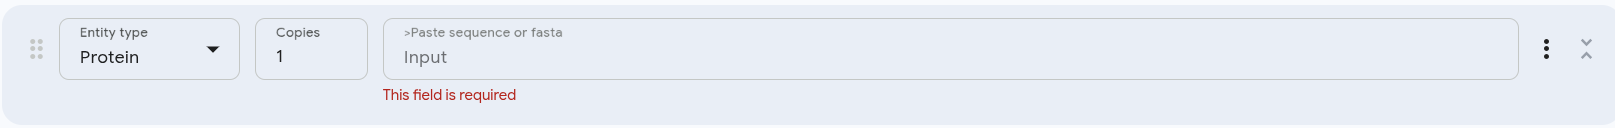
\includegraphics[width=0.95\textwidth]{../figures/af3_etapes/1_champ_vide.png}
  \caption{Étape 4 : la ligne d'entité vide, avant de coller la séquence.}
  \label{fig:af3_champ_vide}
\end{figure}

\begin{figure}[H]
\begin{enumerate}
  \setcounter{enumi}{4}
  \item Coller la séquence. Le serveur l'affiche découpée par blocs de 10, avec la numérotation au-dessus.
\end{enumerate}
  \centering
  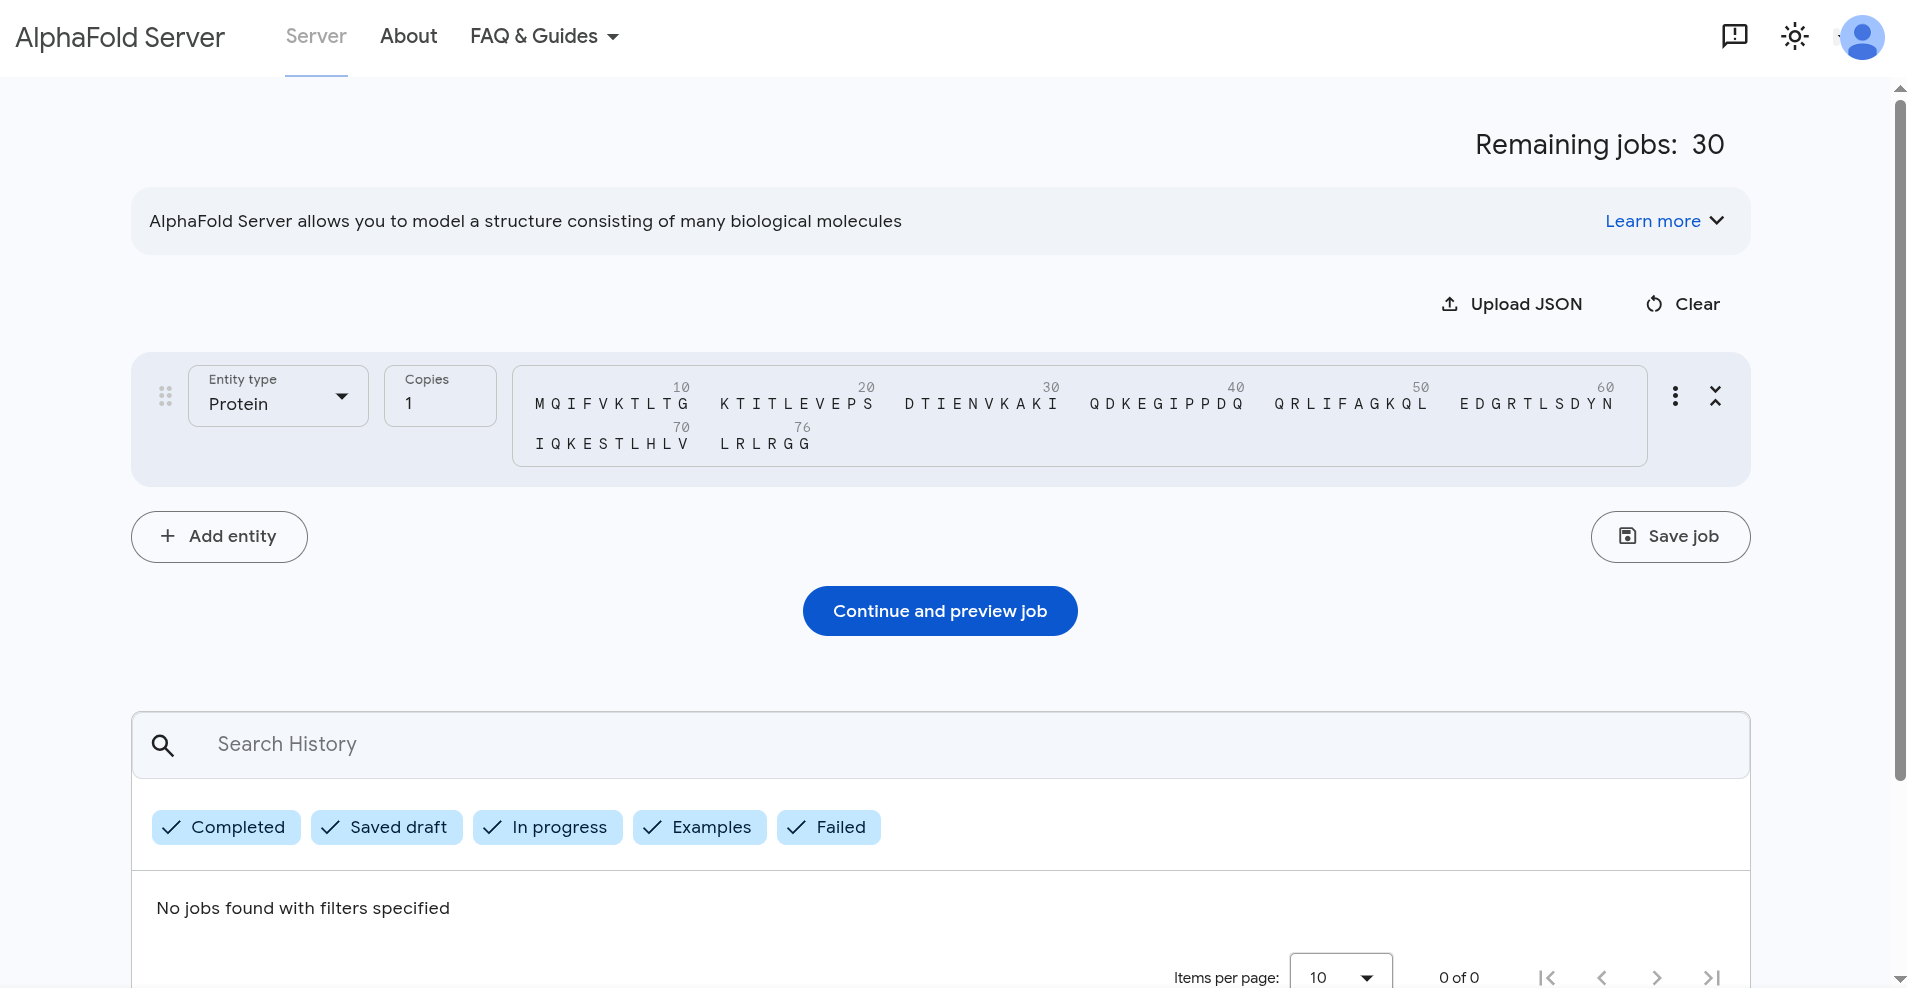
\includegraphics[width=0.95\textwidth]{../figures/af3_etapes/2_sequence_collee.png}
  \caption{Étape 5 : la séquence de la calmoduline collée (149 résidus), prête à être soumise.}
  \label{fig:af3_sequence}
\end{figure}

\begin{figure}[H]
\begin{enumerate}
  \setcounter{enumi}{5}
  \item Cliquer sur le bouton bleu \og Continue and preview job \fg{}. Une fenêtre récapitulative s'ouvre (figure~\ref{fig:af3_preview}) :
  \begin{itemize}
    \item \og Job name \fg{} : le serveur propose un nom (date et heure) ; le remplacer par \texttt{calmoduline} pour retrouver la tâche facilement ;
    \item \og Seed \fg{} : laisser l'interrupteur désactivé (\og Seed: Auto \fg{}), le serveur tire alors une graine au hasard ;
    \item vérifier le tableau : \emph{Protein}, 1 copie, \og (length 149) \fg{}.
  \end{itemize}
  \item Cliquer sur \og Confirm and submit job \fg{}. Le compteur \og Remaining jobs \fg{} diminue de 1.
\end{enumerate}
  \centering
  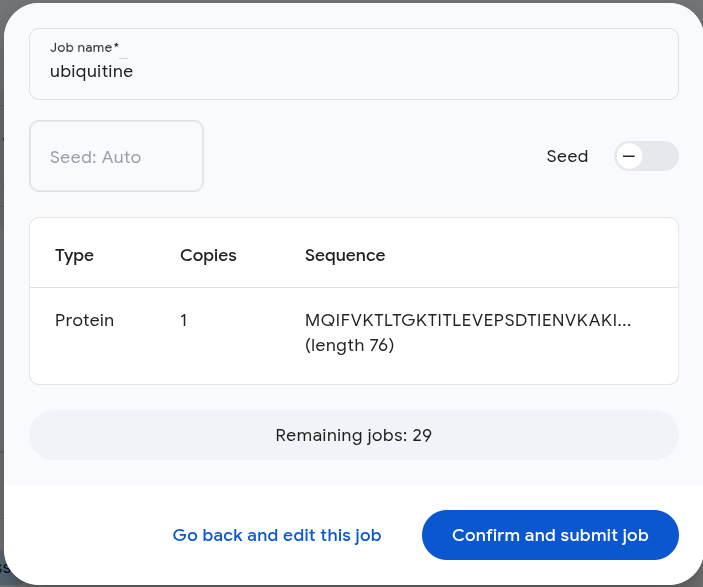
\includegraphics[width=0.55\textwidth]{../figures/af3_etapes/3_previsualisation.png}
  \caption{Étapes 6 et 7 : la fenêtre de prévisualisation avant l'envoi.}
  \label{fig:af3_preview}
\end{figure}

\begin{figure}[H]
\begin{enumerate}
  \setcounter{enumi}{7}
  \item Dans l'historique, sous le formulaire, attendre la fin du calcul (figure~\ref{fig:af3_historique}), puis cliquer sur le nom de la tâche.
\end{enumerate}
  \centering
  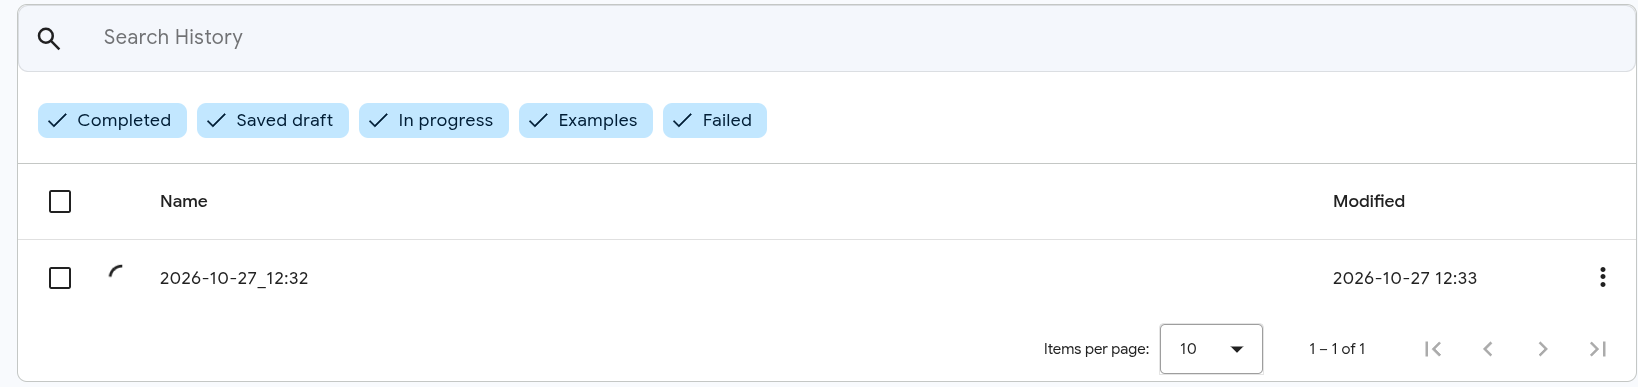
\includegraphics[width=0.95\textwidth]{../figures/af3_etapes/4_historique.png}
  \caption{Étape 8 : une tâche dans l'historique, en cours de calcul (icône de chargement à gauche du nom). La capture montre le premier essai sur l'ubiquitine (annexe~\ref{sec:ubiquitine}), qui avait gardé le nom proposé par défaut.}
  \label{fig:af3_historique}
\end{figure}

\begin{figure}[H]
\begin{enumerate}
  \setcounter{enumi}{8}
  \item Lire le résultat : la légende des couleurs pLDDT et les scores (\og ipTM = - \fg{}, \og pTM = 0.61 \fg{}) en haut, la structure 3D colorée par pLDDT à gauche et la matrice PAE à droite (figure~\ref{fig:af3_calmoduline}).
  \item Cliquer sur \og Download \fg{} et décompresser l'archive dans \texttt{results/}.
\end{enumerate}
  \centering
  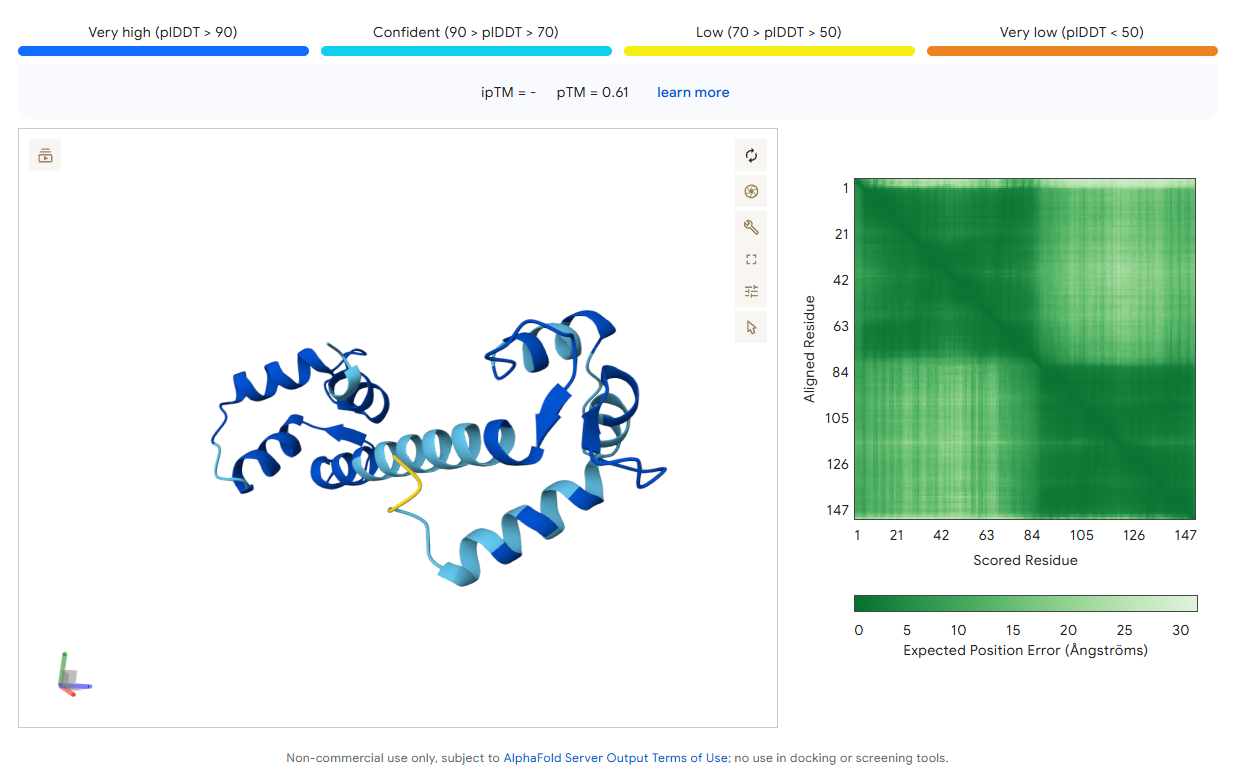
\includegraphics[width=0.95\textwidth]{../figures/af3_calmoduline.png}
  \caption{Résultat d'AlphaFold3 (AlphaFold Server) pour la calmoduline : structure colorée par pLDDT (à gauche), matrice PAE (à droite) ; pTM = 0,61.}
  \label{fig:af3_calmoduline}
\end{figure}
